\begin{figure}[H]
    \centering
    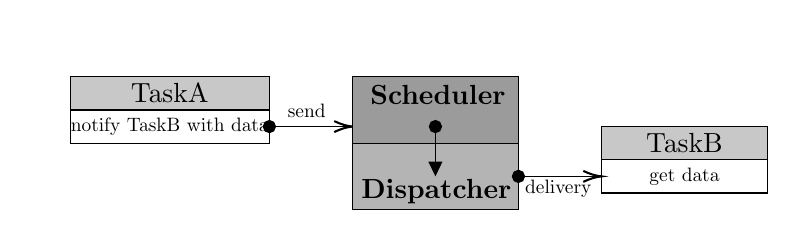
\begin{tikzpicture}[x=0.75pt,y=0.75pt,scale=0.8, yscale=-1]
        \draw   (140,110) -- (260,110) -- (260,130) -- (140,130) -- cycle ;
        \draw    (260,120) -- (308,120) ;
        \draw [shift={(310,120)}, rotate = 180] [color={rgb, 255:red, 0; green, 0; blue, 0 }  ][line width=0.75]    (10.93,-3.29) .. controls (6.95,-1.4) and (3.31,-0.3) .. (0,0) .. controls (3.31,0.3) and (6.95,1.4) .. (10.93,3.29)   ;
        \draw [shift={(260,120)}, rotate = 0] [color={rgb, 255:red, 0; green, 0; blue, 0 }  ][fill={rgb, 255:red, 0; green, 0; blue, 0 }  ][line width=0.75]      (0, 0) circle [x radius= 3.35, y radius= 3.35]   ;
        \draw  [fill={rgb, 255:red, 200; green, 200; blue, 200 }  ,fill opacity=1 ] (140,90) -- (260,90) -- (260,110) -- (140,110) -- cycle ;
        \draw  [fill={rgb, 255:red, 155; green, 155; blue, 155 }  ,fill opacity=1 ] (310,90) -- (410,90) -- (410,130) -- (310,130) -- cycle ;
        \draw  [fill={rgb, 255:red, 180; green, 180; blue, 180 }  ,fill opacity=1 ] (310,130) -- (410,130) -- (410,170) -- (310,170) -- cycle ;
        \draw    (360,120) -- (360,148) ;
        \draw [shift={(360,150)}, rotate = 270] [fill={rgb, 255:red, 0; green, 0; blue, 0 }  ][line width=0.75]  [draw opacity=0] (8.93,-4.29) -- (0,0) -- (8.93,4.29) -- cycle    ;
        \draw [shift={(360,120)}, rotate = 90] [color={rgb, 255:red, 0; green, 0; blue, 0 }  ][fill={rgb, 255:red, 0; green, 0; blue, 0 }  ][line width=0.75]      (0, 0) circle [x radius= 3.35, y radius= 3.35]   ;
        \draw    (410,150) -- (458,150) ;
        \draw [shift={(460,150)}, rotate = 180] [color={rgb, 255:red, 0; green, 0; blue, 0 }  ][line width=0.75]    (10.93,-3.29) .. controls (6.95,-1.4) and (3.31,-0.3) .. (0,0) .. controls (3.31,0.3) and (6.95,1.4) .. (10.93,3.29)   ;
        \draw [shift={(410,150)}, rotate = 0] [color={rgb, 255:red, 0; green, 0; blue, 0 }  ][fill={rgb, 255:red, 0; green, 0; blue, 0 }  ][line width=0.75]      (0, 0) circle [x radius= 3.35, y radius= 3.35]   ;
        \draw   (460,140) -- (560,140) -- (560,160) -- (460,160) -- cycle ;
        \draw  [fill={rgb, 255:red, 200; green, 200; blue, 200 }  ,fill opacity=1 ] (460,120) -- (560,120) -- (560,140) -- (460,140) -- cycle ;
        \draw (200,100) node  [align=left] {TaskA};
        \draw (120,66) node  [align=left] {};
        \draw (361.5,101) node  [align=left] {\textbf{Scheduler}};
        \draw (200,120) node [scale=0.7] [align=left] {notify TaskB with data};
        \draw (282.5,110.5) node [scale=0.7] [align=left] {send};
        \draw (360.5,159) node  [align=left] {\textbf{Dispatcher}};
        \draw (434,157.5) node [scale=0.7] [align=left] {delivery};
        \draw (510,130) node  [align=left] {TaskB};
        \draw (500,146) node  [align=left] {};
        \draw (510,150) node [scale=0.7] [align=left] {get data};
    \end{tikzpicture}
    \caption{A notification used to send an event directly from one task to another}
    \label{fig:simplenotifications}
\end{figure}


